% ── COVER PAGE ──────────────────────────────────────────────
\begin{titlepage}
  \thispagestyle{empty}
	\centering
	\begin{tikzpicture}[remember picture,overlay]
		% تصویر پس‌زمینه که کل صفحه را می‌پوشاند
		\node[inner sep=0pt] at (current page.center) {
			
\includegraphics[width=\paperwidth,height=\paperheight]{tex/cover.png}
		};
		% یک لایه‌ی نیمه‌شفاف برای بهتر خوانده شدن متن
		\fill[white!15!MainBlue, opacity=0.7] ($(current page.north west)+(1cm,-1cm)$) rectangle ($(current page.south east)+(-1cm,+1cm)$);
		
		% خطوط تزئینی
		\draw[AccentGold, line width=3pt] ($(current page.north west)+(1.5cm,-6.5cm)$) -- ($(current page.north east)+(-1.5cm,-6.5cm)$);
		\draw[AccentGold, line width=3pt] ($(current page.north west)+(1.5cm,-14.5cm)$) -- ($(current page.north east)+(-1.5cm,-14.5cm)$);
	\end{tikzpicture}
	
	\vspace*{3.5cm}
	
  {\Huge\bfseries\color{white}\shadow{\Huge طرح نهادی برای گذار دموکراتیک ایران \par}}

	% {\Huge\bfseries\color{white} طرح نهادی گذار ایران \par}
	
	\vspace{1.5cm}
	
	{\huge\bfseries\color{AccentGold} مجلس مهستان \par}
	
	\vspace{0.8cm}
	
	{\Large\color{LightBlue!80} نسخه‌ی بازنگری‌شده‌ی طرح \par}
	
	\vfill
	
	\begin{tcolorbox}[
		enhanced, parbox=false,
		colback=white!10!MainBlue,
		colframe=AccentGold,
		arc=15pt,
		boxrule=1.5pt,
		width=0.8\textwidth,
		left=10pt, right=10pt, top=15pt, bottom=15pt,
		opacityback=0.6
		]
		\centering\color{white}
		\Large\bfseries
	  ترکیب سنجیده‌ی واقعیت و ارزش \\
		\vskip 0.3cm
		\large\mdseries
  بکارگیری هر دو بال تکنوکراسی و دموکراسی برای ساختن ایرانی آزاد و آباد
	\end{tcolorbox}
	
	\vfill
	
	{\large\bfseries\color{white} مهدی سالم \par}
	\vspace{0.2cm}
	{\small\color{LightBlue!60} اسفند ۱۴۰۴ / مارس ۲۰۲۶ \par}
	
	\vspace{1cm}
\end{titlepage}

% ── FRONT MATTER ────────────────────────────────────────────
\frontmatter
\pagestyle{plain}

% ── Abstract / Opening Statement ───────────────────────────
\chapter*{پیش‌گفتار}
\addcontentsline{toc}{chapter}{پیش‌گفتار}
\begin{summarybox}

  این سند چارچوب نهادی پیشنهادی برای دوران گذار دموکراتیک ایران را تشریح می‌کند. محور آن \textbf{«مجلس مهستان»} است — نهادی منتخب و مردم‌محور — که مسئولیت هدایت فرایند گذار را بر عهده می‌گیرد. این طرح بر اصولی استوار است که هدف آن‌ها تضمین انتقال قدرت‌ صلح‌آمیز، حفظ حقوق و آزادی‌های شهروندان، و ایجاد پایه‌ای محکم برای دموکراسی پایدار است.

این سند زنده و پویاست. تمام پیشنهادها، اعداد و ساختارها برای بحث و بازنگری ارائه شده‌اند. تصمیم نهایی درباره‌ی آینده‌ی ایران تنها با \textbf{مردم ایران} است. با این حال، برخی عناصر این طرح بر پایه‌ی اندیشه، تجربه‌های تخصصی و درس‌های آموخته‌شده‌ی جهانی شکل گرفته‌اند و نویسنده بر آن‌ها تأکید دارد؛ از این رو تغییر یا حذف آن‌ها لزوماً مورد تأیید نویسنده نخواهد بود. این موارد در بخش‌های مربوطه به‌طور جداگانه توضیح داده شده‌اند.

در چنین مقاطعی، ملت‌ها با دوگانگی‌ای اساسی روبه‌رو می‌شوند: ۱- آیا باید حق تعیین سرنوشت را به نسل‌های آینده واگذار کنند و آزادی انتخاب آنان را محترم بشمارند، یعنی آیا قوانین اساسی منعطفی برای رژیم سیاسی جدید تنظیم کنند؟، از اصول و بندهای غیر قابل تغییر استفاده نکنند؟ \footnote{ با توجه به این مهم که اصول تخلف ناپذیر در حول و حوش خود، نهادهای ثابت و روابط قدرتی شکل خواهند داد که تغییر آن جز با خشونت و درگیری میسر شدنی نیست!}  یا ۲- باید بر پایه‌ی تجربه‌های به‌دست‌آمده و ضرورت‌های موجود، نقشه‌ی راهی مطمئن و بنیادی استوار برای آیندگان به یادگار بگذارند؟ .\footnote{زیرا هیجان‌ها یا توهم‌های ایشان ممکن است به شکست‌هایی فاجعه‌بار بی‌انجامند و به هزینه‌های غیرضروری و تکرار تجربه‌های تلخی منجر شوند که دستاوردهای یک ملت را و پدران موسس آنرا از میان ببرند.}

آیا تعیین اصولی تخلف‌ناپذیر و دشوار برای تغییر، به معنای تعیین تکلیف و نوعی پدرسالاری برای آیندگان است، یا تصمیمی سنجیده و میراثی گران‌بها که از آزادی، رواداری و تکثر در جامعه محافظت می‌کند؟

\end{summarybox}

\vspace{1cm}
\begin{center}
	{\large\color{MahestanDarkBlue}\itshape
		«ایران برای همه‌ی ایرانیان»}
\end{center}

\newpage
\pagestyle{plain}

\begin{center}
    
\centering
ایده‌های هدایت کننده... 
\begin{tabular}{>{\raggedright\arraybackslash}p{0.4\linewidth}>{\raggedright\arraybackslash}p{0.1\linewidth}>{\raggedleft\arraybackslash}p{0.4\linewidth}}   
\textbf{نه به ...} &  & \textbf{آری به ...} \\
فرد محوری &  & رویه و قانون محوری \\
هم‌قبیلگی محوری &  & هم‌سرنوشتی محوری \\
ایدئولوژی محوری &  & رای و اراده محوری \\
اعتماد محوری &  & شفافیت و تضمین محوری \\
ایمان‌مندی و عقیده‌محوری&  & پرسشگری واندیشه‌محوری  \\
تکلیف و تسلیم محوری &  & حقوق و آزادی محوری \\
فرافکنی و انتظار محوری &  & عاملیت و مشارکت محوری \\
ساده‌اندیشی و خواست محوری &  & هم‌رقصی با پیچیدگی‌ها و ساخت محوری \\
گذشته و سابقه‌محوری &  & سرنوشت و نتیجه‌محوری \\
پدرسالاری و ارباب‌محوری &  & مسئولیت‌مشترک محوری \\
خود رایی و دیکتاتور محوری &  & هم‌فهمی و گفتگو محوری \\

\end{tabular}
\end{center}

% --- Image correctly placed BELOW text ---
\begin{figure}[!htb]
\centering
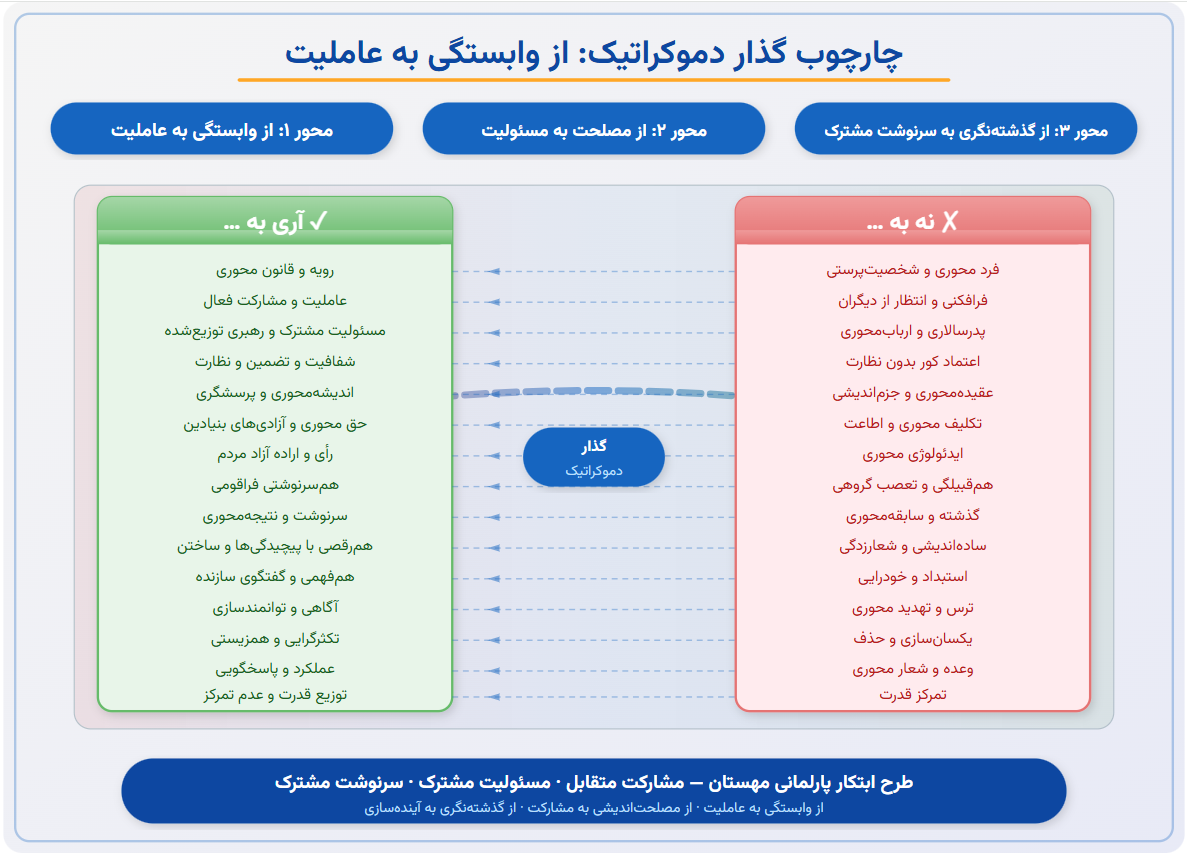
\includegraphics[width=\textwidth, keepaspectratio]{figures/yes-no.png}
\end{figure}

\newpage
\pagestyle{plain}
% ────────────────────────────────────────────────────────────
%  جدول ایده‌های هدایت‌کننده — نه به … / آری به …
% ────────────────────────────────────────────────────────────
\begin{tcolorbox}[
  enhanced,
  breakable,
  colback=white,
  colframe=MahestanBlue,
  arc=6pt,
  boxrule=1.5pt,
  title={\large\bfseries ایده‌های هدایت‌کننده‌ی چارچوب گذار دموکراتیک},
  fonttitle=\bfseries\color{white},
  coltitle=white,
  colbacktitle=MahestanDarkBlue,
  top=1pt, bottom=1pt, left=4pt, right=4pt
]

\centering
\small
\renewcommand{\arraystretch}{1}

\begin{tabularx}{\linewidth}{
  >{\raggedleft\arraybackslash\columncolor{SoftGreen}}X
  c
  >{\raggedleft\arraybackslash\columncolor{SoftRed}}X
}

% ── Header ──────────────────────────────────────────────
\rowcolor{white}
\cellcolor{MahestanGreen!20}
  \textbf{\textcolor{MahestanGreen}{\large ✓ \; آری به …}} &
  &
\cellcolor{MahestanRed!20}
  \textbf{\textcolor{MahestanRed}{\large ✗ \; نه به …}} \\

\midrule

% ── محور اول: از وابستگی به عاملیت ──────────────────────
\rowcolor{MahestanLightBlue!30}
\multicolumn{3}{c}{%
  \textbf{\textcolor{MahestanDarkBlue}{%
    محور اول: از وابستگی به عاملیت}}} \\

\textbf{رویه و قانون محوری}\newline
\scriptsize نهادسازی و اتکا به فرآیندهای شفاف
  & {\color{MahestanBlue}$\Longleftarrow$}
  & \textbf{فرد محوری}\newline
\scriptsize وابستگی به شخصیت‌ها و رهبران فردی \\

\textbf{عاملیت و مشارکت محوری}\newline
\scriptsize شهروندی فعال و پذیرش مسئولیت
  & {\color{MahestanBlue}$\Longleftarrow$}
  & \textbf{فرافکنی و انتظار محوری}\newline
\scriptsize انتظار از دیگران و فرافکنی مسئولیت \\

\textbf{مسئولیت مشترک محوری}\newline
\scriptsize رهبری توزیع‌شده و مسئولیت جمعی
  & {\color{MahestanBlue}$\Longleftarrow$}
  & \textbf{پدرسالاری و ارباب‌محوری}\newline
\scriptsize سلسله‌مراتب و تمرکز اختیار \\

\textbf{توزیع قدرت و عدم‌تمرکز}\newline
\scriptsize تقویت نهادهای محلی و مردمی
  & {\color{MahestanBlue}$\Longleftarrow$}
  & \textbf{تمرکز قدرت}\newline
\scriptsize انحصار تمام قدرت در یک نقطه \\

\midrule

% ── محور دوم: از مصلحت‌اندیشی به مشارکت ────────────────
\rowcolor{MahestanLightBlue!30}
\multicolumn{3}{c}{%
  \textbf{\textcolor{MahestanDarkBlue}{%
    محور دوم: از مصلحت‌اندیشی به مشارکت و مسئولیت}}} \\

\textbf{شفافیت و تضمین محوری}\newline
\scriptsize سازوکارهای قابل‌راستی‌آزمایی و نظارت
  & {\color{MahestanBlue}$\Longleftarrow$}
  & \textbf{اعتماد کور محوری}\newline
\scriptsize اتکا به حسن‌نیت بدون نظارت \\

\textbf{اندیشه‌محوری}\newline
\scriptsize تفکر انتقادی و پرسشگری مستمر
  & {\color{MahestanBlue}$\Longleftarrow$}
  & \textbf{عقیده‌محوری}\newline
\scriptsize پایبندی جزمی به باورهای ثابت \\

\textbf{حق محوری}\newline
\scriptsize تضمین حقوق بنیادین و آزادی‌ها
  & {\color{MahestanBlue}$\Longleftarrow$}
  & \textbf{تکلیف محوری}\newline
\scriptsize تأکید بر اطاعت و وظایف یک‌سویه \\

\textbf{عملکرد و پاسخگویی محوری}\newline
\scriptsize ارزیابی بر اساس نتایج عملی
  & {\color{MahestanBlue}$\Longleftarrow$}
  & \textbf{وعده و شعار محوری}\newline
\scriptsize فریب با شعار و وعده‌های توخالی \\

\textbf{هم‌فهمی و گفتگو محوری}\newline
\scriptsize تصمیم‌گیری مشورتی و سازنده
  & {\color{MahestanBlue}$\Longleftarrow$}
  & \textbf{استبداد و خودرایی}\newline
\scriptsize تصمیم‌گیری یک‌جانبه و حذفی \\

\midrule

% ── محور سوم: از هویت و گذشته به سرنوشت مشترک ──────────
\rowcolor{MahestanLightBlue!30}
\multicolumn{3}{c}{%
  \textbf{\textcolor{MahestanDarkBlue}{%
    محور سوم: از هویت و گذشته‌نگری به منافع و سرنوشت مشترک}}} \\

\textbf{هم‌سرنوشتی محوری}\newline
\scriptsize ساختن آینده‌ای مشترک فراتر از مرزهای قومی
  & {\color{MahestanBlue}$\Longleftarrow$}
  & \textbf{هم‌قبیلگی محوری}\newline
\scriptsize تعلق گروهی و قبیله‌ای \\

\textbf{رأی و اراده محوری}\newline
\scriptsize احترام به رأی جمعی و اراده آزاد
  & {\color{MahestanBlue}$\Longleftarrow$}
  & \textbf{ایدئولوژی محوری}\newline
\scriptsize تحمیل چارچوب ایدئولوژیک واحد \\

\textbf{سرنوشت و نتیجه‌محوری}\newline
\scriptsize نگاه به آینده و ارزیابی بر اساس نتایج
  & {\color{MahestanBlue}$\Longleftarrow$}
  & \textbf{گذشته و سابقه‌محوری}\newline
\scriptsize گیرافتادن در گذشته و داوری بر پایه سوابق \\

\textbf{هم‌رقصی با پیچیدگی‌ها و ساخت محوری}\newline
\scriptsize پذیرش پیچیدگی واقعیت و ساختن تدریجی
  & {\color{MahestanBlue}$\Longleftarrow$}
  & \textbf{ساده‌اندیشی و خواست محوری}\newline
\scriptsize ساده‌سازی مسائل و شعارزدگی \\

\textbf{تکثرگرایی و همزیستی}\newline
\scriptsize جشن تنوع و پذیرش تفاوت‌ها
  & {\color{MahestanBlue}$\Longleftarrow$}
  & \textbf{یکسان‌سازی و حذف}\newline
\scriptsize سرکوب تفاوت‌ها و تحمیل یکدستی \\

\textbf{آگاهی و توانمندسازی}\newline
\scriptsize امنیت از طریق دانایی و مشارکت
  & {\color{MahestanBlue}$\Longleftarrow$}
  & \textbf{ترس و تهدید محوری}\newline
\scriptsize حکمرانی بر پایه ارعاب \\

\bottomrule
\end{tabularx}

\end{tcolorbox}